\chapter{Espín, medición y espacio de estados bidimensional}

\lectureoverview{El espín tiene dirección, pero toda medición de una de sus componentes devuelve solo \(+1\) o \(-1\). Primero formularemos este enigma operacional y luego veremos por qué la lógica ordinaria de conjuntos falla en el caso de mediciones incompatibles. Un espacio vectorial complejo bidimensional proporciona el lenguaje adecuado: las probabilidades se obtienen a partir de amplitudes, las alternativas distinguibles son ortogonales y las bases arriba--abajo, derecha--izquierda y hacia dentro--hacia fuera codifican tres direcciones espaciales sin convertir un vector de estado en una flecha ordinaria.}

\section{Del cúbit al espín}

Al sistema de dos estados que introdujimos como cúbit lo llamaremos ahora \emph{espín}. El cambio de nombre incorpora la dirección espacial a la discusión, pero también crea un peligro con la palabra \emph{vector}. Hay que distinguir dos objetos diferentes:

\begin{definition}
Un \emph{vector tridimensional} es un vector real ordinario en el espacio tridimensional. Sin calificativo, \emph{vector} designará un elemento de un espacio vectorial abstracto, como el espacio complejo de estados que se usa en mecánica cuántica.
\end{definition}

El espín puede prepararse con respecto a un eje del espacio ordinario. Sin embargo, su estado se representará mediante un vector abstracto. La relación entre ambas afirmaciones es una de las cosas que debemos averiguar; no puede darse por sentada a partir de un dibujo.

\section{Por qué no se puede prescindir del aparato}

La mecánica clásica nos lleva a imaginar un observador ideal que obtiene información sobre un sistema perturbándolo tan poco como se quiera. Supongamos, por ejemplo, que queremos ver un objeto macroscópico. Lo iluminamos, recogemos con una lente la luz reflejada y ampliamos la imagen. La luz ejerce cierta fuerza, pero, en la idealización clásica, su intensidad puede reducirse mientras se aumenta la amplificación. Es posible hacer que la perturbación sea arbitrariamente pequeña sin renunciar a la idea de una medición.

Ese procedimiento límite falla en mecánica cuántica. Se puede mejorar, blindar y calibrar un aparato, pero, en general, no es posible hacer que una medición sea a la vez informativa y arbitrariamente no invasiva. Algo del sistema cambia. Esto no significa que toda medición destruya todas las propiedades ni que no se pueda reproducir el resultado. Significa que el aparato forma parte de la pregunta física que se plantea y que no se puede ignorar el estado posterior a la medición.

Por ahora, consideremos que el aparato es una caja negra con dos características: se puede orientar en el espacio y su pantalla registra \(+1\) o \(-1\). Una flecha pequeña en la pizarra es una etiqueta práctica para un espín preparado:

\begin{figure}[htbp]
\centering
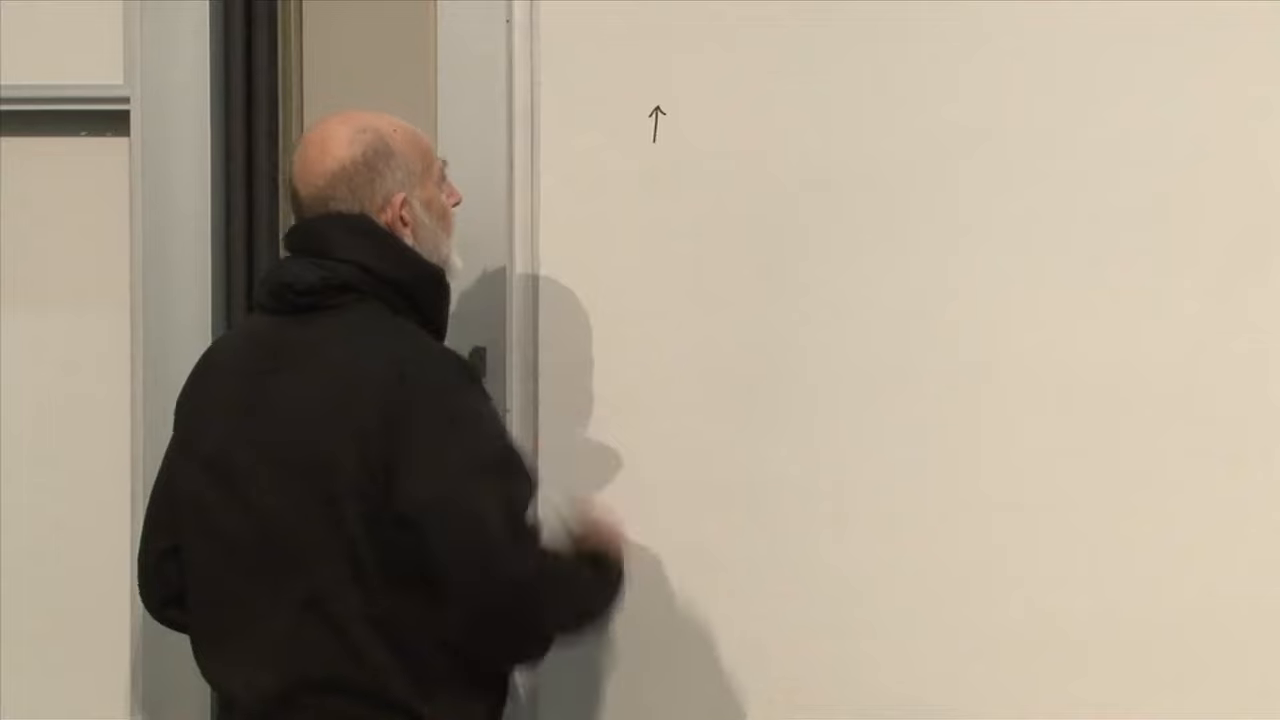
\includegraphics[width=0.64\textwidth]{lecture_02_figure_02.png}
\caption{La primera marca provisional de un espín preparado a lo largo de un eje. La flecha indica una preparación; todavía no es un modelo clásico del estado.}
\lectureframe{00:05:15}
\end{figure}

Elijamos los ejes de modo que \(z\) apunte hacia arriba en la pizarra, \(x\) hacia la derecha y \(y\) hacia fuera de la pizarra. Si el aparato se orienta en la dirección unitaria \(\hat m\), el resultado es
\begin{equation}
\sigma_{\hat m}=\pm1.
\end{equation}
En particular,
\[
\sigma_z=\pm1,\qquad \sigma_x=\pm1,\qquad \sigma_y=\pm1.
\]
En esta etapa, la palabra \emph{componente} tiene un sentido operacional: \(\sigma_z\) es lo que indica el aparato orientado a lo largo de \(z\). Todavía no es la componente según \(z\) de una flecha clásica oculta.

\subsection{Repetibilidad y perturbación}

Supongamos que una medición de \(z\) da \(+1\). Si no hay ninguna operación intermedia, una segunda medición de \(z\) vuelve a dar \(+1\), igual que las repeticiones posteriores. La primera medición ha preparado un estado en el que esa misma pregunta tiene una respuesta definida.

\begin{classroomqa}
\audiencequestion{Si una medición cuántica perturba el espín, ¿por qué una repetición inmediata da el mismo resultado?}
\lecturerresponse{La perturbación no es indiscriminada. Medir \(\sigma_z\) puede cambiar lo que ocurriría en una medición posterior de \(x\) o de \(y\), y aun así dejar reproducible el valor recién medido de \(\sigma_z\). Un experimento útil requiere precisamente esta forma limitada de estabilidad.}
\end{classroomqa}

Giremos ahora el aparato \(180^\circ\). Un espín que dio \(+1\) con la orientación hacia arriba da \(-1\) con la orientación invertida. Si volvemos a poner el aparato en posición vertical, el resultado es \(+1\). Por tanto, la orientación importa. Un termómetro no indicaría una temperatura negativa por el mero hecho de darle la vuelta; el analizador de espín se comporta de otra manera porque plantea una pregunta direccional.

\begin{figure}[htbp]
\centering
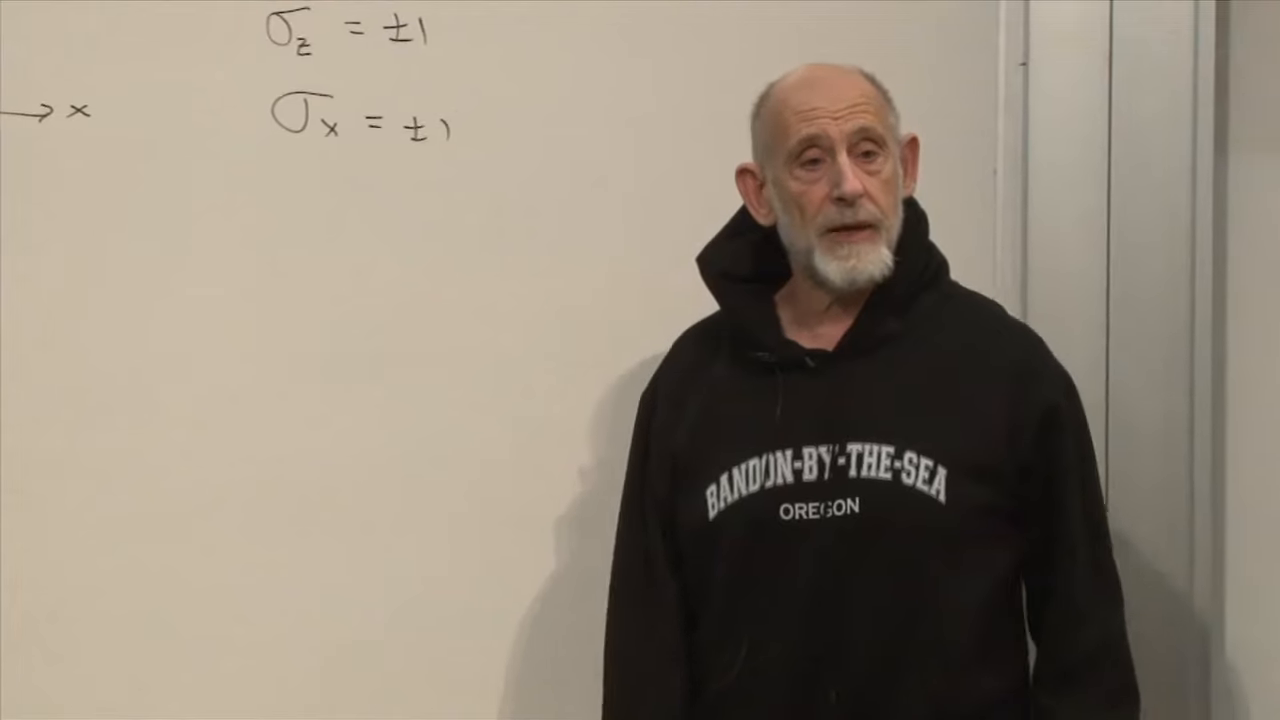
\includegraphics[width=0.72\textwidth]{lecture_02_figure_03.png}
\caption{La pizarra registra las etiquetas de dos valores \(\sigma_z=\pm1\) y \(\sigma_x=\pm1\), junto con la indicación del eje \(x\).}
\lectureframe{00:12:46}
\end{figure}

El contraste con un vector unitario clásico es inmediato. Las componentes clásicas varían continuamente entre \(-1\) y \(+1\). Un vector unitario perpendicular al eje \(x\) tiene componente \(x\) igual a cero. En cambio, un analizador de espín orientado a lo largo de \(x\) nunca muestra cero. Muestra \(+1\) o \(-1\), incluso si el espín se preparó a lo largo de \(z\).

\section{Resultados individuales y promedios de tipo vectorial}

Preparemos un espín obteniendo \(\sigma_z=+1\) y midamos después \(\sigma_x\). La mitad de los ensayos preparados de la misma manera da \(+1\) y la otra mitad da \(-1\). Así pues,
\begin{equation}
\langle \sigma_x\rangle=0.
\end{equation}
La misma preparación da
\begin{equation}
\langle \sigma_y\rangle=0.
\end{equation}
A la inversa, un espín preparado con \(\sigma_x=+1\) tiene probabilidades iguales para los dos resultados de una medición posterior de \(z\) o de \(y\).

En esa afirmación se esconden dos experimentos distintos. Medir repetidamente \(\sigma_x\) sobre el \emph{mismo} espín después del primer resultado \(x\) solo confirma ese resultado. Para obtener la estadística de cincuenta--cincuenta se necesitan muchos espines preparados en el mismo estado \(z\), o bien devolver repetidamente un espín a esa misma preparación antes de cada medición de \(x\).

\begin{classroomqa}
\audiencequestion{¿Qué ocurre si no se ha preparado deliberadamente un espín antes de que entre en el aparato?}
\lecturerresponse{El resultado sigue siendo \(+1\) o \(-1\), pero sus probabilidades dependen del estado que tenga realmente el espín. La preparación es el procedimiento controlado que permite comparar ensayos repetidos. Si ocurre una manipulación desconocida entre dos mediciones, ya no se garantiza la repetibilidad; si no ocurre nada, el resultado de medir la misma componente es reproducible.}
\end{classroomqa}

\subsection{Dos direcciones arbitrarias}

Preparemos el espín a lo largo de una dirección unitaria \(\hat n\) obteniendo \(+1\) con un analizador orientado a lo largo de \(\hat n\). Midamos luego a lo largo de otra dirección unitaria \(\hat m\). Cada ensayo sigue dando solo \(\pm1\), pero el promedio de ensayos preparados de la misma manera es
\begin{equation}
\boxed{\langle\sigma_{\hat m}\rangle=\hat n\cdot\hat m
=\cos\theta_{nm}.}
\label{eq:spin-average}
\end{equation}
En la pizarra se usa la notación abreviada \(\langle\sigma_m\rangle=n\cdot m\):

\begin{figure}[htbp]
\centering
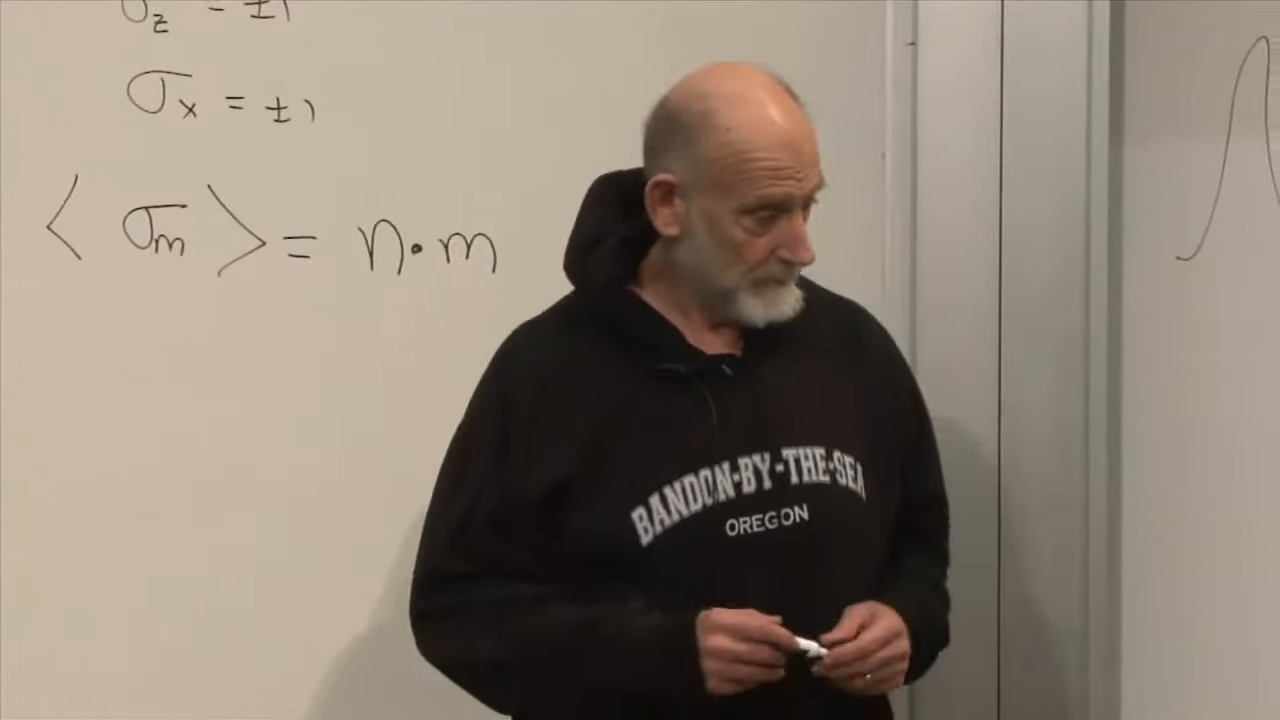
\includegraphics[width=0.74\textwidth]{lecture_02_figure_04.png}
\caption{La ley de tipo vectorial corresponde al promedio del conjunto, no a un resultado individual \(\pm1\).}
\lectureframe{00:23:22}
\end{figure}

La ecuación~\eqref{eq:spin-average} incluye los casos anteriores. Si \(\hat m=\hat n\), el promedio es \(+1\); como ningún resultado puede superar \(+1\), todos los ensayos dan \(+1\). Si \(\hat m=-\hat n\), todos dan \(-1\). Para ejes perpendiculares, el promedio es cero y las frecuencias son iguales.

Si \(p_+\) y \(p_-\) denotan las probabilidades de los dos resultados posibles, entonces
\[
p_++p_-=1,\qquad p_+-p_-=\hat n\cdot\hat m.
\]
Por consiguiente,
\begin{equation}
p_\pm=\frac{1\pm\hat n\cdot\hat m}{2}.
\label{eq:direction-probabilities}
\end{equation}
\editorialnote{La lección enuncia los dos resultados y su media. La ecuación~\eqref{eq:direction-probabilities} se deduce directamente de esos dos hechos.}

\begin{classroomqa}
\audiencequestion{¿La cantidad entre corchetes angulares es un \emph{valor esperado} o un promedio ordinario?}
\lecturerresponse{Es la media de los resultados registrados en muchas repeticiones. \emph{Valor esperado} es la terminología estándar, pero aquí no se pretende indicar ningún tipo adicional de promedio. El aparato produce una lista de valores \(+1\) y \(-1\); los corchetes denotan la media aritmética de esa lista en el límite de un conjunto grande.}
\end{classroomqa}

\begin{classroomqa}
\audiencequestion{¿Tenía ya la flecha \(\hat n\) un significado geométrico antes de conocer la ley del promedio?}
\lecturerresponse{Al principio era una etiqueta para indicar la orientación del aparato de preparación. El experimento de inversión y la dependencia del promedio respecto de \(\hat n\cdot\hat m\) dan a esa etiqueta un significado geométrico operacional. El aparato define el significado de las componentes; un resultado individual nunca proporciona una proyección clásica.}
\end{classroomqa}

Esta es la primera conciliación entre la imagen direccional y los datos discretos. El espín individual no se comporta como una flecha clásica con componentes de valores continuos. Sin embargo, la estadística de muchos espines preparados de la misma manera se transforma exactamente como las componentes de un vector unitario tridimensional.

\section{Proposiciones clásicas como conjuntos}

Antes de construir el espacio de estados cuánticos, consideremos cómo funciona la lógica en un sistema clásico. Sea \(\Omega\) el conjunto de estados posibles. Una proposición \(A\) se representa mediante el subconjunto de estados para los que \(A\) es verdadera.

Para un dado de seis caras,
\[
A=\{2,4,6\}
\]
puede representar \emph{el resultado es par}, mientras que
\[
B=\{4,5,6\}
\]
puede representar \emph{el resultado es mayor que tres}. Las operaciones lógicas se convierten en operaciones entre conjuntos:
\begin{equation}
\neg A=A^c,\qquad
A\land B=A\cap B,\qquad
A\lor B=A\cup B.
\label{eq:classical-logic}
\end{equation}
Aquí \(\lor\) es la disyunción inclusiva: \(A\lor B\) es verdadera cuando \(A\) es verdadera, cuando \(B\) es verdadera o cuando ambas lo son. No es el uso cotidiano exclusivo de \emph{o bien \(A\) o \(B\), pero no ambos}.

\begin{classroomqa}
\audiencequestion{Una medición de espín solo tiene dos resultados, pero la dirección de preparación varía continuamente. ¿El conjunto de estados es finito o continuo?}
\lecturerresponse{El conjunto de direcciones de preparación posibles es continuo, aunque todo analizador elegido tenga solo dos lecturas. Precisamente por eso, contar las etiquetas del detector no basta para describir el espacio de estados.}
\end{classroomqa}

Para los subconjuntos clásicos, la intersección y la unión no dependen del orden en que se mencionen las proposiciones:
\[
A\cap B=B\cap A,\qquad A\cup B=B\cup A.
\]
Por tanto, es posible idealizar una prueba experimental de una proposición clásica compuesta sin incorporar un orden a la lógica.

\section{Una prueba de la disyunción que depende del orden}

Consideremos las proposiciones cuánticas
\begin{equation}
A:\sigma_z=+1,\qquad B:\sigma_x=+1.
\end{equation}
Cada proposición tiene una prueba clara. Orientar el aparato a lo largo de \(z\) permite comprobar \(A\), y orientarlo a lo largo de \(x\) permite comprobar \(B\). El problema aparece cuando se intenta verificar \(A\lor B\) poniendo a prueba una proposición y, si resulta falsa, poniendo a prueba la otra.

Imaginemos que un preparador invisible ha suministrado un espín hacia arriba según \(z\). Si se comprueba primero \(A\), el resultado es con certeza \(+1\) y la prueba de la disyunción termina con \emph{verdadera}.

Invirtamos el orden. Comprobar primero \(B\) da
\[
P(B)=\frac12,\qquad P(\neg B)=\frac12.
\]
Si \(B\) es falsa, la medición de \(x\) ha preparado, pese a todo, un estado definido de \(x\). Al comprobar \(A\) en ese estado se obtiene
\[
P(A\mid \neg B)=\frac12,\qquad
P(\neg A\mid \neg B)=\frac12.
\]
Por tanto, el procedimiento invertido informa que ambas proposiciones son falsas con probabilidad
\begin{equation}
P(\neg B\ \text{then}\ \neg A)
=\frac12\cdot\frac12=\frac14.
\end{equation}
Con un orden, la disyunción siempre se acepta; con el otro, se rechaza en una cuarta parte de los ensayos.

\begin{classroomqa}
\audiencequestion{¿Se debe la contradicción simplemente a que ignoramos el estado preparado en secreto?}
\lecturerresponse{No. Se eligió esa preparación oculta únicamente para que la comparación fuera clara. La primera medición de \(x\) prepara físicamente un estado de \(x\), de modo que la prueba posterior de \(z\) se realiza sobre un estado que ha cambiado. Dar al observador más información sobre la preparación inicial no deshace esa intervención.}
\end{classroomqa}

\begin{classroomqa}
\audiencequestion{¿Se podría comprobar la disyunción mediante una jerarquía de preguntas más elaborada, en vez de usar esta regla secuencial?}
\lecturerresponse{Desde luego, se pueden definir distintos procedimientos experimentales, pero entonces se trata de mediciones cuánticas distintas. No hay un subconjunto \(A\cup B\) independiente del procedimiento cuya verdad se limite a descubrir sin tener en cuenta el aparato. La dependencia del orden advierte que la lógica clásica de conjuntos no es la lógica propia de estas proposiciones.}
\end{classroomqa}

Más adelante, las proposiciones se representarán mediante operadores de proyección. La advertencia algebraica concisa es
\begin{equation}
P_A P_B\ne P_B P_A.
\end{equation}
Por ahora no hace falta nada más de la teoría de operadores. Lo importante es que las pruebas incompatibles no conmutan y que sus proposiciones compuestas no se pueden tratar como uniones ordinarias de conjuntos.

\begin{classroomqa}
\audiencequestion{¿Se puede organizar una versión de este experimento con dos partículas de modo que la elección de la prueba actúe hacia atrás en el tiempo?}
\lecturerresponse{Esa pregunta requiere herramientas que aún no hemos desarrollado. La secuencia con un solo espín no permite concluir nada sobre una causalidad hacia atrás, así que la cuestión queda abierta en vez de responderse con conjeturas.}
\end{classroomqa}

\section{El espacio vectorial de estados}

Un conjunto contiene elementos, pero, por lo general, no hay una manera natural de sumar dos elementos para obtener un tercero. Un espacio vectorial lineal tiene más estructura. Si \(\ket{A}\) y \(\ket{B}\) son vectores y \(\alpha,\beta\in\mathbb C\), entonces
\begin{equation}
\alpha\ket{A}+\beta\ket{B}
\end{equation}
es otro vector del mismo espacio. Los estados cuánticos se representan en un espacio lineal complejo de este tipo.

Para cada ket \(\ket{A}\) hay un bra dual correspondiente \(\bra{A}\). Al emparejar un bra con un ket se obtiene un número complejo: el producto interno. Este satisface la simetría conjugada,
\begin{equation}
\braket{A}{B}=\braket{B}{A}^{*}.
\label{eq:conjugate-symmetry}
\end{equation}

\begin{figure}[htbp]
\centering
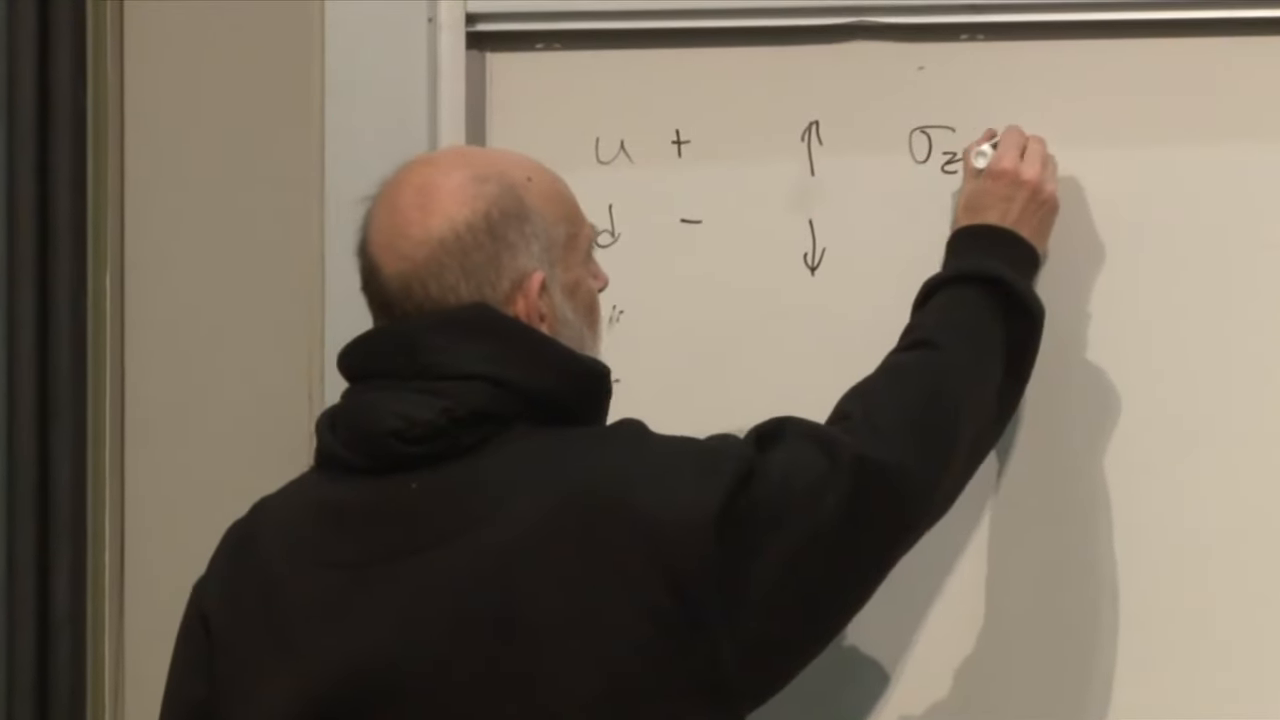
\includegraphics[width=0.78\textwidth]{lecture_02_figure_05.png}
\caption{La pizarra resume las combinaciones lineales y la inversión conjugada de un producto interno.}
\lectureframe{00:46:53}
\end{figure}

La longitud al cuadrado de un vector es
\begin{equation}
\|\ket{A}\|^2=\braket{A}{A}.
\end{equation}
La ecuación~\eqref{eq:conjugate-symmetry} hace que este número sea igual a su propio conjugado complejo y, por tanto, real; los axiomas del producto interno también garantizan que sea no negativo. Dos vectores son ortogonales cuando
\begin{equation}
\braket{A}{B}=0.
\end{equation}
La dimensión del espacio es el máximo número de direcciones no nulas mutuamente ortogonales que se pueden elegir.

\begin{classroomqa}
\audiencequestion{¿Toda base debe estar formada por vectores mutuamente ortogonales?}
\lecturerresponse{No. Una base solo tiene que ser linealmente independiente y generar el espacio. Las bases ortogonales son especialmente prácticas porque es fácil obtener los coeficientes y las probabilidades. En dos dimensiones, dos vectores no paralelos pueden formar una base aunque su producto interno no sea cero.}
\end{classroomqa}

\section{El espacio bidimensional del espín}

Se postula que el espacio de estados de un espín es un espacio vectorial complejo bidimensional,
\begin{equation}
\mathcal H_{\mathrm{spin}}\cong\mathbb C^2.
\end{equation}
Hay continuamente muchos vectores de estado posibles, pero solo hacen falta dos vectores de base independientes para expresar cualquiera de ellos.

Empecemos con los estados preparados por un aparato orientado según \(z\):
\begin{align}
\ket{u}&\longleftrightarrow \sigma_z=+1,\\
\ket{d}&\longleftrightarrow \sigma_z=-1.
\end{align}
Las letras \(u,d\), los signos \(+,-\) y las flechas \(\uparrow,\downarrow\) son etiquetas alternativas para las mismas dos preparaciones. Como una medición de \(z\) los distingue con certeza, sus vectores de estado son ortogonales:
\begin{equation}
\braket{u}{d}=0.
\end{equation}
Elijamos que tengan longitud unitaria,
\[
\braket{u}{u}=\braket{d}{d}=1.
\]

Entonces, todo estado de espín se puede escribir como
\begin{equation}
\ket{A}=\alpha_u\ket{u}+\alpha_d\ket{d},
\qquad \alpha_u,\alpha_d\in\mathbb C.
\label{eq:general-spin-state}
\end{equation}
La regla de probabilidad es
\begin{equation}
P(u|A)=|\alpha_u|^2,\qquad
P(d|A)=|\alpha_d|^2.
\label{eq:born-z}
\end{equation}
Como necesariamente debe ocurrir uno de los dos resultados,
\begin{equation}
|\alpha_u|^2+|\alpha_d|^2=1.
\label{eq:normalization}
\end{equation}

\begin{figure}[htbp]
\centering
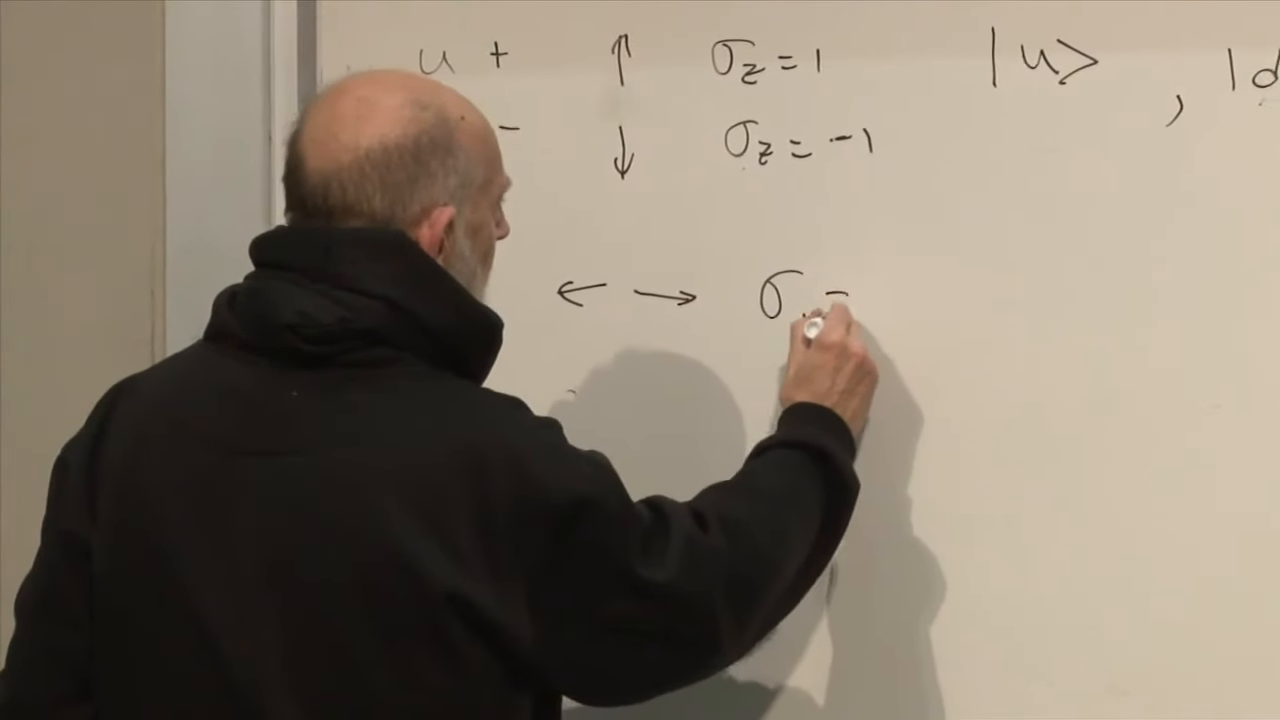
\includegraphics[width=0.78\textwidth]{lecture_02_figure_06.png}
\caption{Una expansión general en los estados arriba--abajo, la suma de las probabilidades de los dos resultados y la condición equivalente de norma unitaria.}
\lectureframe{01:03:38}
\end{figure}

La equivalencia con la normalización unitaria se deduce directamente:
\begin{align}
\braket{A}{A}
&=(\alpha_u^*\bra{u}+\alpha_d^*\bra{d})
  (\alpha_u\ket{u}+\alpha_d\ket{d})\\
&=|\alpha_u|^2\braket{u}{u}
 +\alpha_u^*\alpha_d\braket{u}{d}\\
&\quad +\alpha_d^*\alpha_u\braket{d}{u}
 +|\alpha_d|^2\braket{d}{d}\\
&=|\alpha_u|^2+|\alpha_d|^2=1.
\end{align}
Así pues, un estado puro físico se representa mediante un vector normalizado.

\begin{classroomqa}
\audiencequestion{¿Estas afirmaciones se están deduciendo o son postulados?}
\lecturerresponse{En este punto son las reglas que se ajustan a los experimentos. El espacio bidimensional, la regla de probabilidad y la interpretación de la ortogonalidad se introducen de manera heurística. Ahora se puede comprobar que son mutuamente coherentes; a continuación se desarrollará la relación sistemática entre estados y observables.}
\end{classroomqa}

\subsection{La ortogonalidad como distinguibilidad}

El contenido físico de la ortogonalidad resulta más útil que la imagen de flechas perpendiculares:

\begin{quote}Los estados que se pueden distinguir con certeza mediante una medición se representan con vectores ortogonales.
\end{quote}

Los estados arriba y abajo cumplen este criterio. Si el estado es arriba, el aparato de \(z\) nunca indica abajo, y viceversa. Un solapamiento distinto de cero indica que un estado puede producir a veces un resultado asociado con el otro.

\section{Base derecha--izquierda}

Sean \(\ket{r}\) y \(\ket{l}\) los estados con espín \(x\) definido:
\[
\ket{r}\longleftrightarrow\sigma_x=+1,\qquad
\ket{l}\longleftrightarrow\sigma_x=-1.
\]
Como el espacio es bidimensional, cada uno debe ser una combinación lineal de \(\ket{u}\) y \(\ket{d}\). Un espín preparado hacia la derecha da arriba y abajo con probabilidades iguales, así que los dos coeficientes deben tener el mismo módulo. Elijamos la convención de fase más sencilla:
\begin{equation}
\ket{r}=\frac{1}{\sqrt2}\bigl(\ket{u}+\ket{d}\bigr).
\label{eq:right-state}
\end{equation}
El aparato de \(x\) distingue con certeza los estados derecha e izquierda, por lo que el estado izquierda debe ser ortogonal al estado derecha. Una elección conveniente es
\begin{equation}
\ket{l}=\frac{1}{\sqrt2}\bigl(\ket{u}-\ket{d}\bigr).
\label{eq:left-state}
\end{equation}
En efecto,
\begin{align}
\braket{l}{r}
&=\frac12(\bra{u}-\bra{d})(\ket{u}+\ket{d})\\
&=\frac12(1-1)=0.
\end{align}

\begin{figure}[htbp]
\centering
\includegraphics[width=0.82\textwidth]{lecture_02_figure_07.png}
\caption{La construcción completa de derecha--izquierda: módulos iguales para arriba--abajo, signos relativos opuestos y producto interno nulo.}
\lectureframe{01:12:15}
\end{figure}

El signo menos global de \(\ket{l}\) es convencional. Sustituir \(\ket{l}\) por \(-\ket{l}\) no cambia ninguna de sus probabilidades. Al sumar y restar las ecuaciones~\eqref{eq:right-state} y~\eqref{eq:left-state} se obtiene el cambio de base inverso:
\begin{align}
\ket{u}&=\frac{1}{\sqrt2}\bigl(\ket{r}+\ket{l}\bigr),\\
\ket{d}&=\frac{1}{\sqrt2}\bigl(\ket{r}-\ket{l}\bigr).
\end{align}
La simetría es importante. Partiendo de la base de \(x\), un estado arriba o abajo es una superposición con pesos iguales de derecha e izquierda, del mismo modo que un estado derecha o izquierda es una superposición con pesos iguales de arriba y abajo.

\section{La base hacia dentro--hacia fuera y la fase relativa}

Orientemos el aparato según \(y\), perpendicular a la pizarra. Escribamos
\[
\ket{i}\longleftrightarrow\sigma_y=+1,\qquad
\ket{o}\longleftrightarrow\sigma_y=-1,
\]
donde la etiqueta del ket \(i\) significa \emph{hacia dentro} y el \(i\) sin adornos que multiplica un ket sigue siendo la unidad imaginaria.

Las probabilidades iguales para arriba y abajo requieren coeficientes de igual módulo. La ortogonalidad entre hacia dentro y hacia fuera requiere una fase relativa que anule su solapamiento. Una elección simétrica es
\begin{align}
\ket{i}&=\frac{1}{\sqrt2}\bigl(\ket{u}+i\ket{d}\bigr),\\
\ket{o}&=\frac{1}{\sqrt2}\bigl(\ket{u}-i\ket{d}\bigr).
\label{eq:in-out-states}
\end{align}
En la base \((u,d)\), los seis estados son
\begin{align}
\ket{u}&=\binom10,
&
\ket{d}&=\binom01,
\\
\ket{r}&=\frac1{\sqrt2}\binom11,
&
\ket{l}&=\frac1{\sqrt2}\binom1{-1},
\\
\ket{i}&=\frac1{\sqrt2}\binom1{i},
&
\ket{o}&=\frac1{\sqrt2}\binom1{-i}.
\end{align}

\begin{figure}[htbp]
\centering
\includegraphics[width=0.82\textwidth]{lecture_02_figure_08.png}
\caption{Los seis vectores columna en la base arriba--abajo. El par inferior difiere en el signo de la fase imaginaria relativa.}
\lectureframe{01:20:50}
\end{figure}

La conjugación compleja en el bra es esencial para comprobar la ortogonalidad:
\begin{align}
\braket{i}{o}
&=\frac12(\bra{u}-i\bra{d})(\ket{u}-i\ket{d})\\
&=\frac12\bigl(1+(-i)(-i)\bigr)=0.
\end{align}

\begin{classroomqa}
\audiencequestion{¿Elegir \(+i\) para \emph{hacia dentro} en vez de \emph{hacia fuera} codifica la orientación de los ejes espaciales?}
\lecturerresponse{Se ha introducido una convención, cuyo significado geométrico se aclarará cuando se desarrollen las matrices de Pauli y las rotaciones. Por ahora, el par debe ser ortogonal y guardar una relación simétrica con las otras bases; intercambiar las etiquetas o invertir el eje \(y\) cambia la convención, pero no la coherencia de la construcción.}
\end{classroomqa}

\subsection{Comprobación de la simetría en la base derecha--izquierda}

Usemos
\[
\ket{u}=\frac{\ket{r}+\ket{l}}{\sqrt2},\qquad
\ket{d}=\frac{\ket{r}-\ket{l}}{\sqrt2}
\]
en el estado hacia dentro:
\begin{align}
\ket{i}
&=\frac1{\sqrt2}
\left(
\frac{\ket{r}+\ket{l}}{\sqrt2}
+i\frac{\ket{r}-\ket{l}}{\sqrt2}
\right)\\
&=\frac{1+i}{2}\ket{r}
 +\frac{1-i}{2}\ket{l}.
\label{eq:in-in-rl}
\end{align}
Aunque ninguno de los coeficientes contenga visiblemente \(1/\sqrt2\),
\begin{equation}
\left|\frac{1+i}{2}\right|^2
=\left|\frac{1-i}{2}\right|^2
=\frac12.
\end{equation}

\begin{figure}[htbp]
\centering
\includegraphics[width=0.82\textwidth]{lecture_02_figure_09.png}
\caption{El cambio de base explícito para el estado hacia dentro y la comprobación de que cada probabilidad en derecha--izquierda es \(1/2\).}
\lectureframe{01:29:10}
\end{figure}

Así pues, cada estado de una de las tres bases da probabilidades iguales cuando se mide en cualquiera de las otras dos. Las bases \(z\), \(x\) y \(y\) son mutuamente no sesgadas.

\section{Por qué hay tres pares de bases distinguidos}

\begin{classroomqa}
\audiencequestion{¿Puede haber un cuarto par de estados relacionado con estos tres pares de manera tan simétrica como lo están entre sí?}
\lecturerresponse{No en un sistema de dos estados. Una vez fijados los tres pares mutuamente no sesgados, no hay un cuarto par con la misma relación de solapamiento igual. La existencia de tres etiquetas espaciales de este tipo está ligada a las tres dimensiones del espacio ordinario, aunque el espacio complejo de estados tenga dimensión dos.}
\end{classroomqa}

Esta conexión se aprecia contando los parámetros físicos. Una columna general
\[
\binom{\alpha_u}{\alpha_d}
\]
contiene dos números complejos y, por tanto, cuatro números reales. La normalización elimina uno:
\[
|\alpha_u|^2+|\alpha_d|^2=1.
\]
Multiplicar ambas componentes por una fase común no cambia ninguna probabilidad de medición:
\begin{equation}
\ket{A}\sim e^{i\chi}\ket{A}.
\label{eq:global-phase}
\end{equation}
Eso elimina un parámetro real más. Por tanto,
\begin{equation}
4-1-1=2
\end{equation}
quedan parámetros reales físicos, exactamente el número de ángulos necesarios para especificar una dirección en el espacio tridimensional.

Un representante conveniente hace explícita la relación:
\begin{equation}
\ket{\psi(\theta,\phi)}
=\cos\frac{\theta}{2}\,\ket{u}
+e^{i\phi}\sin\frac{\theta}{2}\,\ket{d}.
\label{eq:bloch-parameterization}
\end{equation}
\editorialnote{La ecuación~\eqref{eq:bloch-parameterization} es el representante normalizado estándar de la familia de dos parámetros identificada en la lección. Se incluye la forma explícita con semiángulos para concretar el recuento de parámetros; su interpretación dinámica y rotacional corresponde a lecciones posteriores.}

\begin{classroomqa}
\audiencequestion{¿Cuál es la formulación matemática precisa de ignorar la fase global?}
\lecturerresponse{Todos los vectores normalizados del conjunto \(\{e^{i\chi}\ket{\psi}\}\) representan el mismo estado físico. Se identifican esos vectores como equivalentes, de manera parecida a como se considera un único punto físico a varios puntos relacionados por una redundancia declarada. La fase relativa entre componentes sigue siendo medible; solo se descarta la fase que multiplica al vector entero.}
\end{classroomqa}

\begin{classroomqa}
\audiencequestion{¿Se pueden usar en un cálculo vectores no normalizados o con componentes negativas?}
\lecturerresponse{Sí. El álgebra lineal los admite, y un vector intermedio no tiene por qué representar todavía un estado físico preparado. Al final se puede normalizar cualquier vector no nulo. Las componentes negativas y complejas son amplitudes, no probabilidades negativas; las probabilidades se obtienen de los módulos al cuadrado una vez normalizado el estado.}
\end{classroomqa}

\begin{classroomqa}
\audiencequestion{¿Qué ocurre con esta imagen en espacios de dimensión mayor o para espinores más complejos?}
\lecturerresponse{Los mismos principios lineales siguen siendo válidos, pero la relación entre la dimensión del espacio de estados, las rotaciones espaciales y el espín observable se vuelve más rica. Esa extensión queda fuera de la construcción actual de dos estados.}
\end{classroomqa}

\section{La ortogonalidad no es perpendicularidad espacial}

La palabra \emph{ortogonal} tiene ahora un significado abstracto y operacional. No debe confundirse con el ángulo entre dos flechas dibujadas en el espacio ordinario. Las direcciones espaciales arriba y abajo son opuestas, pero los vectores de estado \(\ket{u}\) y \(\ket{d}\) son ortogonales. Las direcciones espaciales arriba y derecha son perpendiculares, pero
\begin{equation}
\braket{u}{r}=\frac1{\sqrt2}\ne0.
\end{equation}

\begin{classroomqa}
\audiencequestion{¿Cómo pueden ser ortogonales las direcciones espaciales opuestas, mientras que las direcciones espaciales perpendiculares no lo son?}
\lecturerresponse{El solapamiento en el espacio de estados mide la distinguibilidad experimental, no el ángulo euclidiano entre las etiquetas. Un único experimento de medición de \(z\) permite distinguir con certeza arriba y abajo, por lo que su solapamiento es nulo. No se pueden distinguir de ese modo arriba y derecha: un espín preparado hacia la derecha a veces da el resultado arriba. Por eso sus vectores de estado tienen solapamiento.}
\end{classroomqa}

La misma idea tiene un análogo en la probabilidad clásica. Dos distribuciones de probabilidad con soportes disjuntos son perfectamente distinguibles: un resultado observado permite identificar cuál de las dos distribuciones se usó. Las distribuciones con soportes que se solapan no pueden distinguirse sin error a partir de una sola muestra. La ortogonalidad cuántica desempeña el papel de la ausencia de solapamiento, mientras que un producto interno distinto de cero indica que algunos resultados son compatibles con cualquiera de las dos preparaciones.

\begin{classroomqa}
\audiencequestion{¿Se debe visualizar el espacio bidimensional de estados como el plano físico que contiene las flechas arriba y derecha?}
\lecturerresponse{No. Las etiquetas \(x,y,z\) se refieren a orientaciones del aparato en el espacio ordinario. Los kets pertenecen a un espacio vectorial complejo con su propio producto interno. El recuento de parámetros conecta ambas estructuras, pero identificarlas punto por punto confundiría la perpendicularidad espacial con la ortogonalidad en el espacio de estados.}
\end{classroomqa}

\section{Estados, mediciones y lo que queda por hacer}

Hasta ahora, la construcción ha consistido en ajustar vectores a hechos operacionales. Las tres orientaciones del aparato etiquetan tres pares de estados normalizados, y los productos internos reproducen las probabilidades observadas. Aún hace falta un tratamiento riguroso que explique cómo actúa un observable como \(\sigma_z\) sobre un estado y por qué sus posibles resultados son sus valores propios. Ese es el siguiente paso.

Ahora puede plantearse con mayor precisión el acertijo lógico anterior. Las proposiciones corresponden a subespacios o a sus proyectores, y los proyectores incompatibles no conmutan. La prueba de la disyunción OR, cuyo resultado dependía del orden, no era una paradoja verbal; fue una primera manifestación de esta estructura no conmutativa.

\begin{classroomqa}
\audiencequestion{Si el estado no es una flecha ordinaria, ¿por qué las tres etiquetas \(x,y,z\) y el promedio \(\langle\sigma_{\hat m}\rangle\) parecen tan clásicos?}
\lecturerresponse{El vector clásico aparece en los promedios de conjuntos. Un solo espín da una respuesta discreta, mientras que muchos espines preparados de forma idéntica producen promedios que se transforman como las componentes de una dirección. El comportamiento clásico macroscópico emerge cuando las grandes colecciones hacen que esos promedios sean estables; no debe interpretarse al revés como un valor continuo oculto en cada espín individual.}
\end{classroomqa}

\begin{classroomqa}
\audiencequestion{¿Es la redundancia de fase común un ejemplo de invariancia gauge?}
\lecturerresponse{Es una invariancia sencilla bajo una fase común y anticipa ideas gauge más generales. Desarrollar aquí esa conexión excedería el alcance de la construcción actual, así que basta con retener la afirmación físicamente pertinente: la fase común es imperceptible; la fase relativa, no.}
\end{classroomqa}

Por último, no debe imaginarse una medición como si simplemente revelara un valor que el espín hubiera llevado consigo desde siempre, en el sentido clásico. La medición prepara el estado asociado al resultado registrado. Por tanto, una repetición inmediata de la misma medición es coherente, mientras que un nuevo conjunto de espines preparados de forma idéntica muestra la distribución de probabilidad que determinan las amplitudes pertinentes. La descripción matemática de esa preparación y de la lectura del resultado será precisa cuando se introduzcan los observables como operadores.